\section{UAV and deployment unit}\label{sec:DeploymentUnit(UAV)}

The UAV is a custom-built, 1.77 m wingspan hexacopter, controlled by a Pixhawk flight controller running ArduPilot Mega flight software. The UAV has a 3DR GPS module using the UBlox NEO-7 chipset.


 The deployment mechanism allows the UAV to carry four SeismicDarts in a circular array, and release them when it reaches the desired GPS location, one at a time.
 The rear of the dart has a circular tip that locks into the deployment mechanism, and rests on a rectangular slot-path. 
 A servomotor rotates the dart tips through the rectangular slot-path, allowing darts to release from a circular opening,  as shown in Fig.~\ref{fig:deployment_system}.



\begin{figure} \centering
  {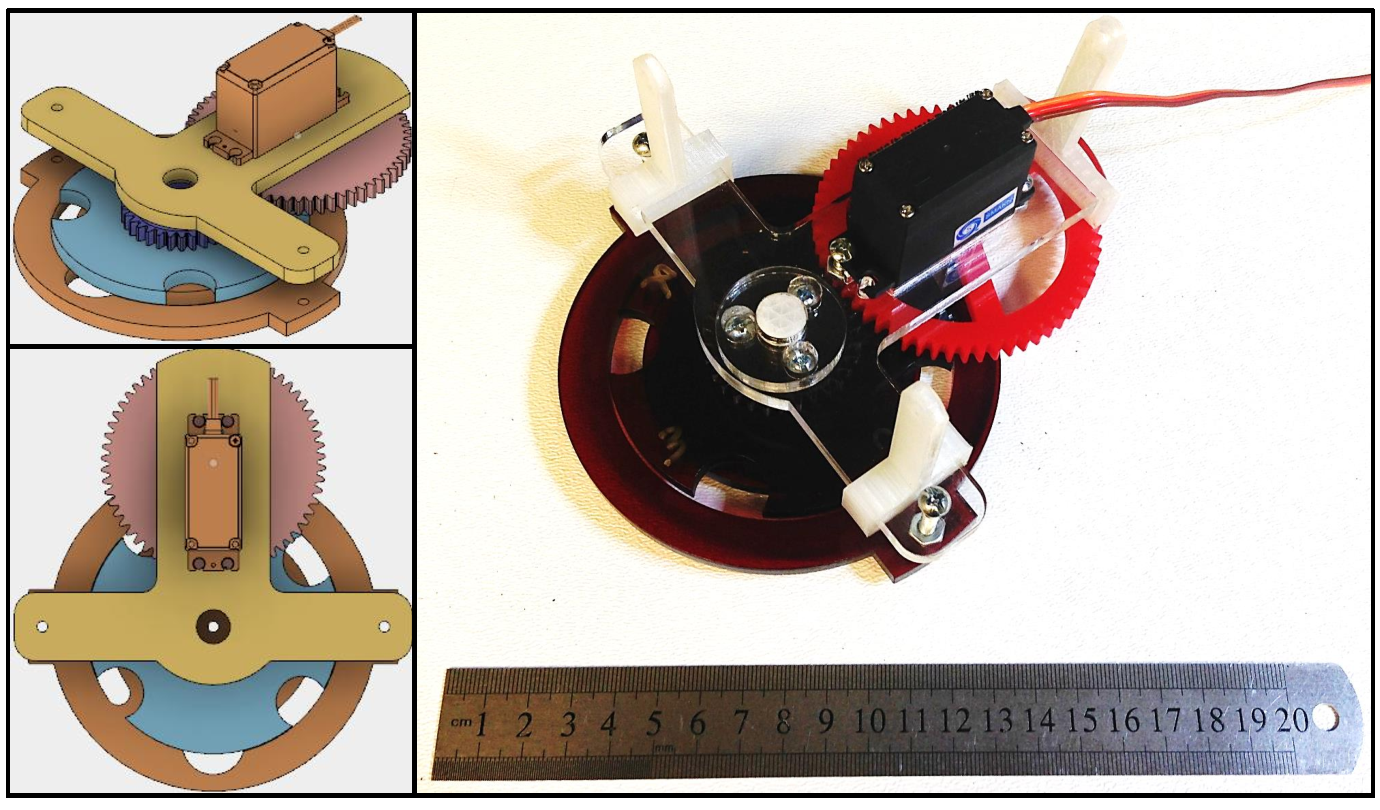
\includegraphics[width=\columnwidth]{deployment_system.pdf}}
 \caption{Deployment system for dropping SeismicDarts from the UAV. Pictured design holds four darts, but can be scaled according to the UAV's carrying capacity.} 
 \label{fig:deployment_system}
\end{figure}




\subsection{Autonomous drop demonstration and accuracy}

The current UAV can place a SeismicDart within $\pm1$ m of the desired location.  
This range is within tolerances for seismic surveys because often features (rocks, water, etc.) exist that require this amount of error from theoretically assigned locations and some survey designs include a random placement component to improve noise cancellation.
%(3) this error minimally perturbs the data since seismic waves travel at 600 m/s near the surface, so a one-meter inaccuracy equates to $\approx$1.6 ms delay.
%(4) the response of a receiver to seismic vibrations is an average over a number of meters.  ?? what does this mean??

To accurately perform a seismic survey, the sensors do not need to placed accurately, but their position must be known within $\approx$ 0.01 m. 
 Knowledge of the exact location compensates for placement inaccuracy.
 Localization can be achieved by placing an RTK GPS in each dart.  A lower-cost solution would use an RTK GPS on the SeismicDrone and perform image registration with the downward facing camera.  As shown in the multimedia attachment, even at a 25 m drop height a planted dart occupies dozens of pixels, enabling cm-level localization accuracy.


%allows corrections for jitter in signal arrival times due to  placement inaccuracy.


%Exp 4: Automatic drop from drone, accuracy in placement
\begin{figure} \centering
  {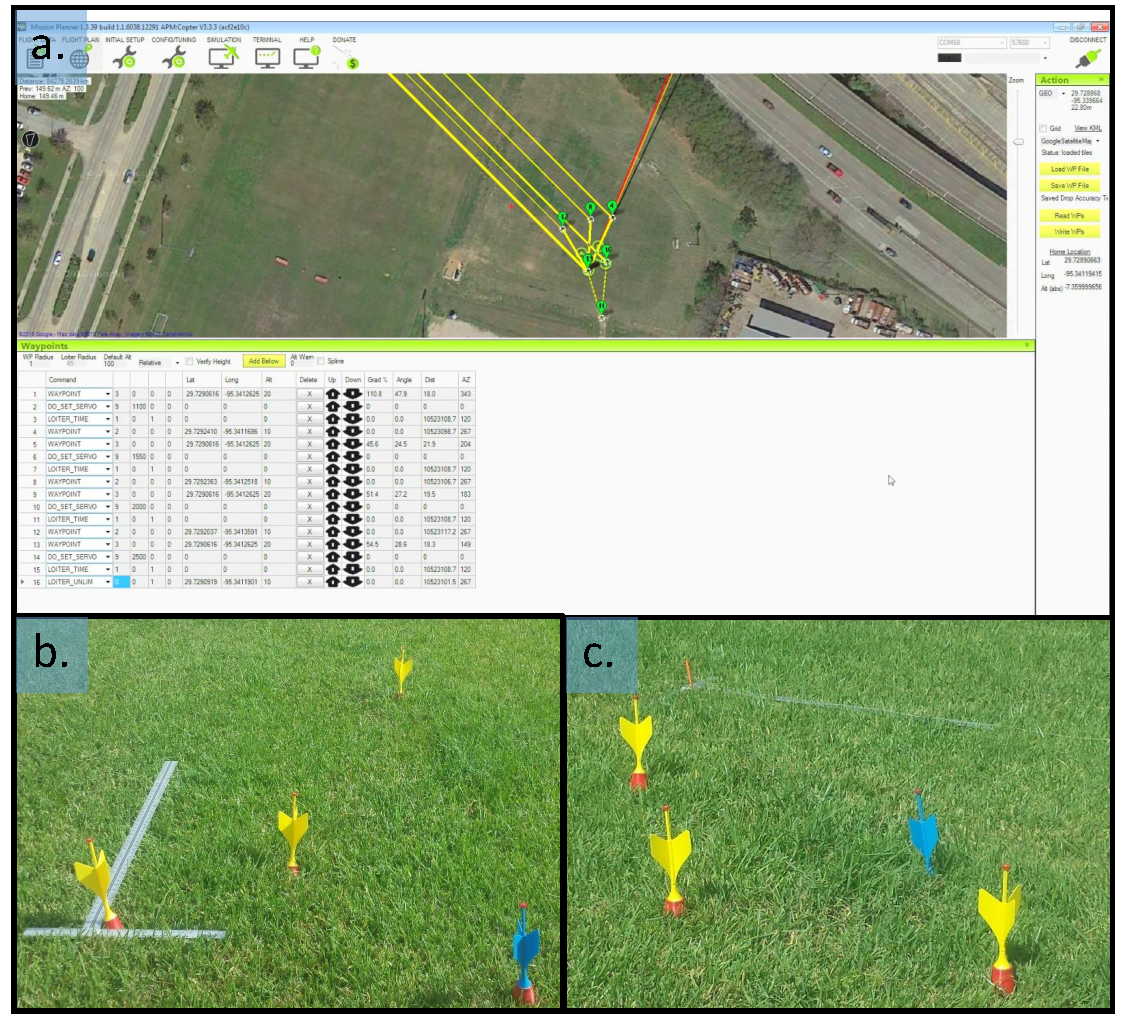
\includegraphics[width=\columnwidth]{accuracy_test_overview.pdf}}
 \caption{a.) Flight plan of accuracy test. b.) First set of darts with reference axes. c.) Third dart set. } 
 \label{fig:Accu_test_darts}
\end{figure}

For the accuracy test, six sets of darts, four darts in each set, were dropped on the same GPS waypoint. Between each drop, the UAV traveled to a nearby GPS waypoint to cancel out the flight controller's stable hover.  This path is shown in Fig.~\ref{fig:Accu_test_darts}a. The UAV then returned to the launch platform to be reloaded, we recorded the dart landing positions, collected the darts, and reloaded the darts on the UAV for the next deployment set.
  Results are shown in Fig.~\ref{fig:SD_accu.pdf}.
  
%To measure position, one dart was picked from the first set as the reference point (the lower left in Fig.~\ref{fig:Accu_test_darts}b), hence the first data point was (0,0). A 1-m T-square was placed with the origin at the dart's drop point to establish reference axes.


 %A rod was placed in the position of the first dart to keep reference as shown in Fig.~\ref{fig:Accu_test_darts}c. 
% The T-square was kept in place and mason twine was suspended to lengthen the reference axes. 
% Future deployments were measured  using the reference point and axes. 



\begin{figure} \centering
  {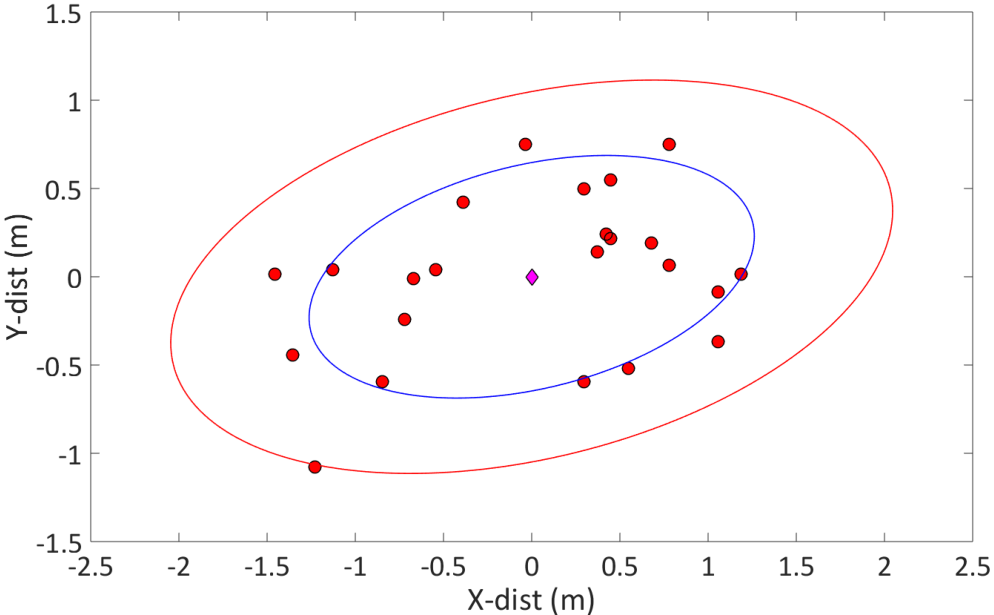
\includegraphics[width=\columnwidth]{SD_accu.pdf}}
 \caption{Targeting accuracy.  Circles show landing locations of 24 darts, each commanded to drop at the same GPS location. The mean position is marked by a diamond, ellipses show  $\sigma$ and 2$\sigma$ covariance.
 \label{fig:SD_accu.pdf}}
\end{figure}


\subsection{Height vs. penetration depth}
%Exp 5: Height vs. penetration depth

FAA rules require that UAVs fly below 400 feet (122 m). Our highest drop tests were from 25 m, and resulted in well-planted geophones on a compacted field with density 4 kg/cm$^2$. Harder soils may require faster impact velocity, so this section examines possible impact velocities as a function of drop height.
For ease of analysis, we will assume the SeismicDart has a constant coefficient of drag $C_d$ and that the drag force is proportional to velocity squared and equal to $\frac{1}{2} v^2 \rho A C_d$, where $v$ is the velocity, $A$ the cross-sectional area and $\rho$ the density of air.  
 The tests were performed near sea level, so $\rho \approx 1.225~\text{kg/m}^3$.
  The dart body is 0.06 m in diameter so $A=0.028$ m$^2$.  We will assume the dart $C_d$ is between that of a streamlined body $C_d=0.04$ and that of an arrow $C_d=1.5$~\cite{miyazaki2013aerodynamic}, and choose that of a sphere $C_d=0.47$.
The terminal velocity is then
\begin{align}
v_T = \sqrt{\frac{2 m g}{\rho A  C_d}} \approx 59 \text{ m/s.}
\end{align}
The velocity at impact is a function of the drop height $h$.
\begin{align}
v_{impact} = v_T  \sqrt{ 1 - e^{ -\frac{\rho A  C_d}{m} h }} \approx 59\sqrt{ 1 - e^{ -0.008 h }} \text{ m/s}
\end{align}
With  $C_d=0.47$, our drop from 25 m achieves only 43\% the terminal velocity (21.1 m/s), and for $C_d=0.04$ only 13\% terminal velocity  (22.0 m/s).
%This implies our tests are far from the limits of the SeismicDart's per
%This implies the SeismicDart is suitable even for much harder soils than tested thus far.
Dropping from the maximum FAA height of 122 m would generate an impact velocity of 39 m/s with $C_d=0.47$,  enabling penetration of harder soils.

\subsection{Robustness}
  The darts are robust. One of the darts used for the shot gather in Fig.~\ref{fig:shotgather_auto_drop} was a veteran of 120 drops.
The most damage observed occurred when we dropped a SeismicDart 10 m onto a bed of  rocks, each approximately  0.1 m in diameter. The steel spike of the dart was blunted, but this damage was quickly compensated by resharpening with a hand file and the SeismicDart was ready to redeploy.


%\begin{figure} \centering
%  {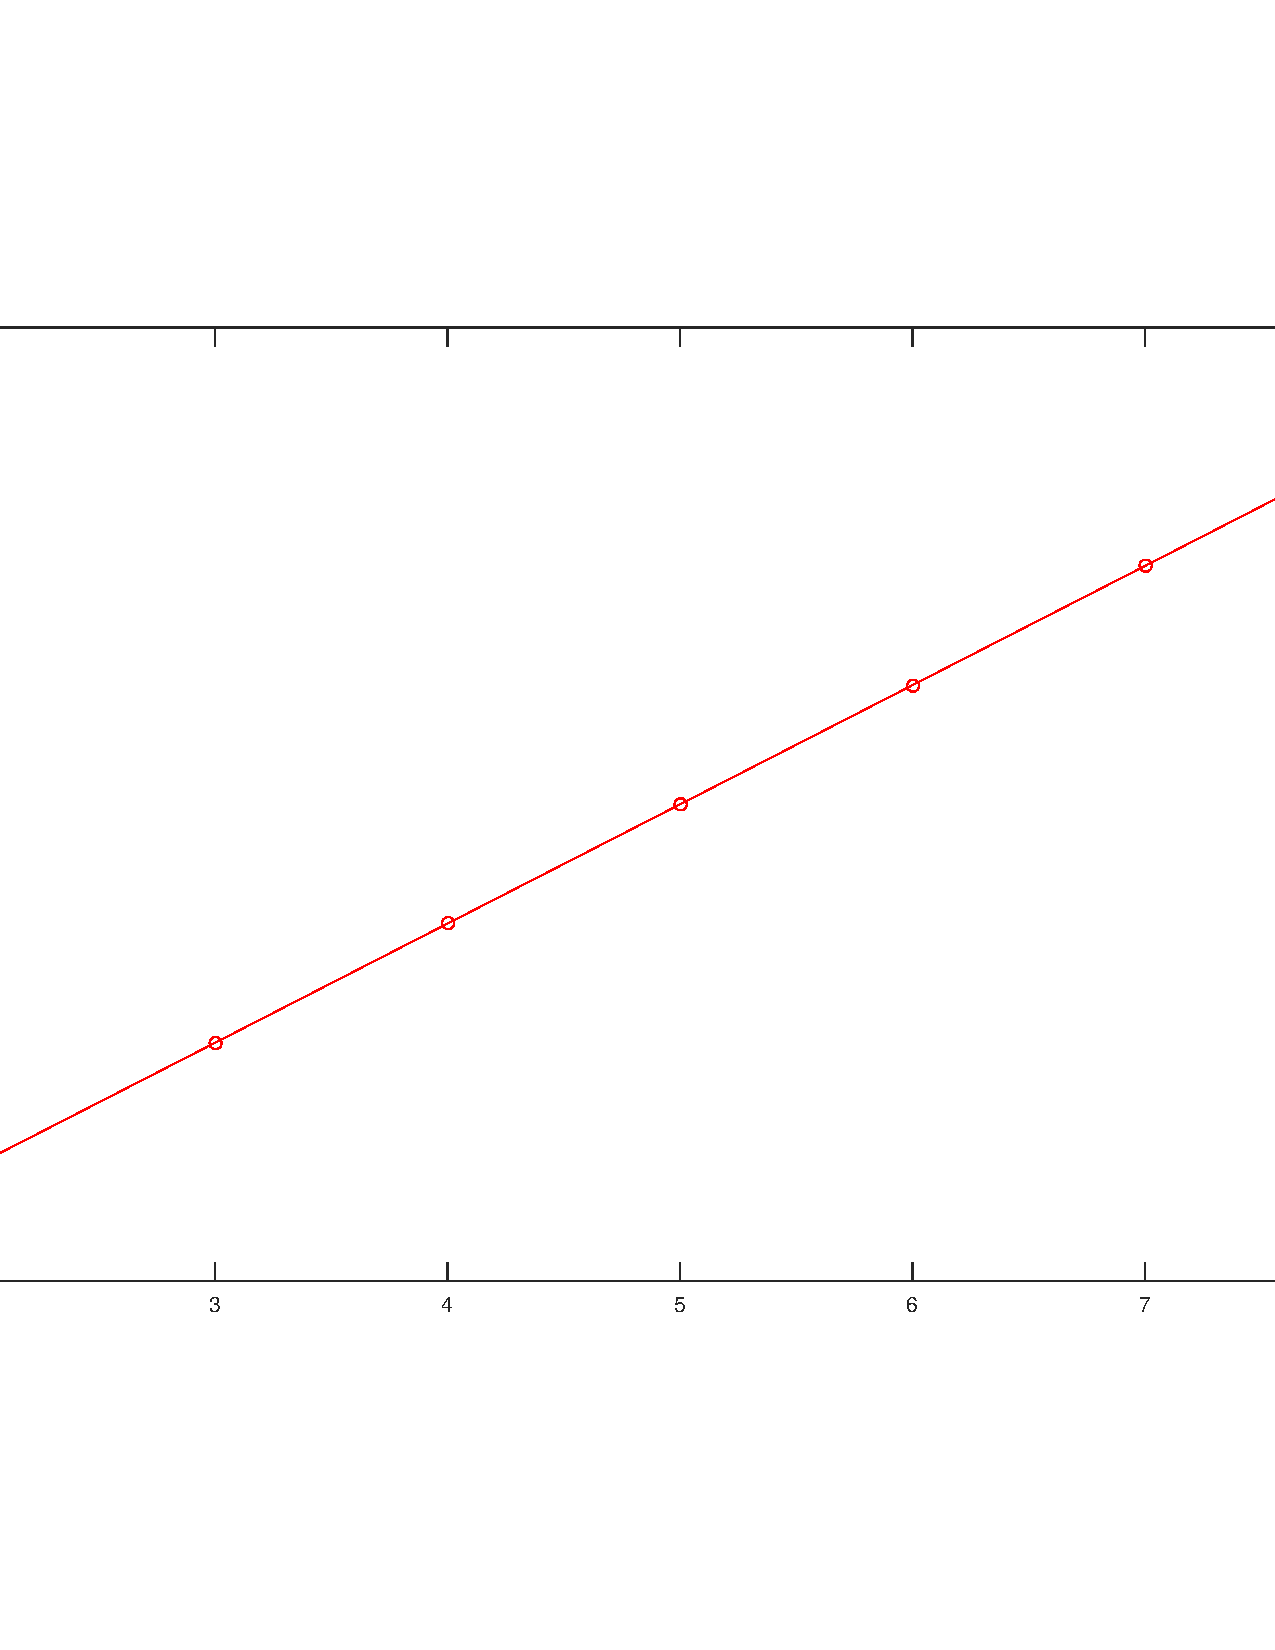
\includegraphics[width=\columnwidth]{replace_graph.pdf}}
% \caption{Plot of pneumatic cannon firing angle vs ending angle} 
% \label{fig:TradvsAutoDrop}
%\end{figure}





